\documentclass{IEEEtran}
\usepackage{graphicx}

\graphicspath{{./figures/}}

\title{Integrating 3D Localization and Haptic Feedback for Interactive Graphics Manipulation}

\author{Armon Shariati, Camillo Jose Taylor}

\begin{document}
\setlength{\pdfpagewidth}{8.5in}
\setlength{\pdfpageheight}{11 in}
\maketitle

\begin{abstract}
    Most virtual reality systems generally fall into one of two categories:
    graphics oriented - which focus on developing immersive environments but
    generally fail to provide users with a strong sense of interactivty - and
    haptics oriented - which focus on constructing tools for touch-based
    manipulation and auditory interaction but tend to be very specialized
    applications and tightly bound device ecosystems. We present our approach
    to creating immersive graphical settings with a high degree of interactive
    manipulation using any number of haptic devices.
\end{abstract}

\section{Introduction}
\label{sec:introduction}

Virtual reality has commanded the attention of the media and the public for
decades, and in recent years the serious attention of researchers worldwide.
French playwright Antonin Artaud is first credited for coining the term
``virtual reality'' in his 1938 book \emph{The Theater and Its Double}. He uses
the term to describe theater, whereby it is a reality that is both illusory and
purely fictitious \cite{website:popularizeVR}. Technology has a come a long way
since Artuad, and our means for creating such extensional realities are ever
expanding. The allure of VR, in the contemporary sense, according to Michael
Abrash of Valve, is that ``presence is an incredibly powerful sensation, and
it's unique to VR; there is no way to create it in any other medium''
\cite{website:steampowered}.  Many devices over the years try to impart the
feeling of presence, but to do so is no trivial task. However, while VR has
long been not much more than an elusive science fiction, recent advancements in
hardware and computing power elevate its prospects to an attainable and
not-so-distant future. 

Gaming is the most obvious example of where VR might find application, and
consequently receives the most attention.  The ability to create immersive
amenable worlds which are a direct extension of our own environments are seen
to yield significant applications medicine and defense as well, among others.
In a recent study at the Department of Surgery at Yale University, researchers
found that surgical residents who receive VR training for laparoscopic
cholecystectomy are able to perform gallbladder dissections 29\% faster than
the control group. Furthermore, non-VR-trained residents are nine times more
likely to transiently fail to make progress and five times more likely to
injure the gallbladder \cite{seymour2002virtual}.

The United States military uses fully immersive virtual simulation training
systems for soldiers in Fort Bragg, N.C. \cite{website:army}. They found that
``the ability to train with this system allows the ``reset'' time to be cut
down, which allows the ability to get more repetitions in a shorter amount of
time and the ability to review each mission on a television screen to enhance
the after action review process upon completion of each mission''.  The VR
system lends itself to having a mutable nature as well. ''The Semi-Automated
Forces Works station gives the trainer the option to create additional static
items like furniture and buildings or items that are animated such as dogs and
birds, inside the virtual world. There can also be modifications made during
the scenario like adding an improvised explosive device or more vehicles and
combatants.''

Head mounted devices (HMDs), grew to become the most popular device for
delivering the VR experience for gamers.  These wearable devices track the
orientation of your head and use the measurements from their on board sensors
such as accelerometers and gyroscopes to adjust the pose of a virtual camera to
correspond to the real time movement of your head.  The first of such devices
include Nintendo's Virtual Boy, Virtual i-O i-glasses, and the VFX-1 Headgear
from Forte Tech. While all very groundbreaking for their time, they are all
plagued with the same problem as the countless HMD devices to follow, in that
the processing power can not contend with what the graphics demand.  In
addition to low resolution displays and limited communication bandwidth, the VR
experience these devices provide are limited at best and would often cause
users to feel sick after a session \cite{zachara2009challenges}. The most
contemporary versions of these devices however, show a great deal of promise.
The Oculus Rift \cite{website:oculusvr} has experienced meteoric success since
debuting in 2012; it has raised \$2.5 million in its opening kickstarter
campaign and receives praise and support from gaming giants including John
Carmack of id Software and Michael Abrash \cite{website:kickstarterovr}.
Although the attention does not go unwarranted since among the many things that
make the device so powerful, it is the first device of its kind to carefully
address the issue of tracker latency. How the Oculus does so will be explained
in Section \ref{sec:hmd}.

The progress made thus far creating visually immersive environments are
degraded if users have no robust means of interaction. Much research has
already been done developing haptic devices to interact with VR systems and
many of them are rather impressive. Examples of large commercial haptic systems
to experience great success include the CyberGrasp glove
\cite{website:cybergrasp} and the Phantom Omni \cite{website:geomagic}.
However, advanced haptic devices such as these are rarely seen interfaced with
the immersive graphical environments being developed in the game industry.
Conversely, while the gaming world focuses on developing graphic solutions, the
haptic devices used to interact with the generated scenes such as the Nintendo
Wiimote \cite{website:wiimote} are fairly one-dimensional input controllers
designed to simulate certain aspects of the experience. Although I should be
mention, that since the introduction of the Oculus, few companies have
attempted to develop more advanced haptic ancillary input and haptic devices
such as the Virtuix Omni - an omnidirectional treadmill and Razer Hydra - a
haptic controller \cite{website:razer}, they still fail to convey the same
level of interactivity as the more cutting edge devices seen in the more
general haptics field.

Ultimately, there still exists a great divide between the graphic solutions and
haptic solutions as far as integration. While some systems attempt to close the
loop from perception, to interaction, to haptic feedback, they often make it
difficult to introduce other tools into their ecosystem such as the more
advanced graphics displays. Moreover, many of these systems would also have
great difficulty providing as large of a virtual space as required for some
military applications and provide as much precision for fine manipulations
tasks such as surgical training.

I present a solution for developing immersive and interactive VR environments,
which allows developers to efficiently leverage large scale motion capture
systems in order to interface any number of haptic devices with a cutting edge
graphics pipeline, to achieve seamless interactivity between users and their
virtual realities. My design also allows my system to interface with robotic
systems as well, which could lead to interesting teleoperation and telepresence
applications. In Section \ref{sec:hmd}, I describe my usage of the Oculus as
the head mounted display. In Section \ref{sec:mocap}, I give an explanation of
how I use motion capture in my system. In Section \ref{sec:results}, I describe
the final simulation. Finally, In Section \ref{sec:future}, I outline the
direction the system should take in the future.

\section{Head Mounted Display}
\label{sec:hmd}

\begin{figure}[]
\centering
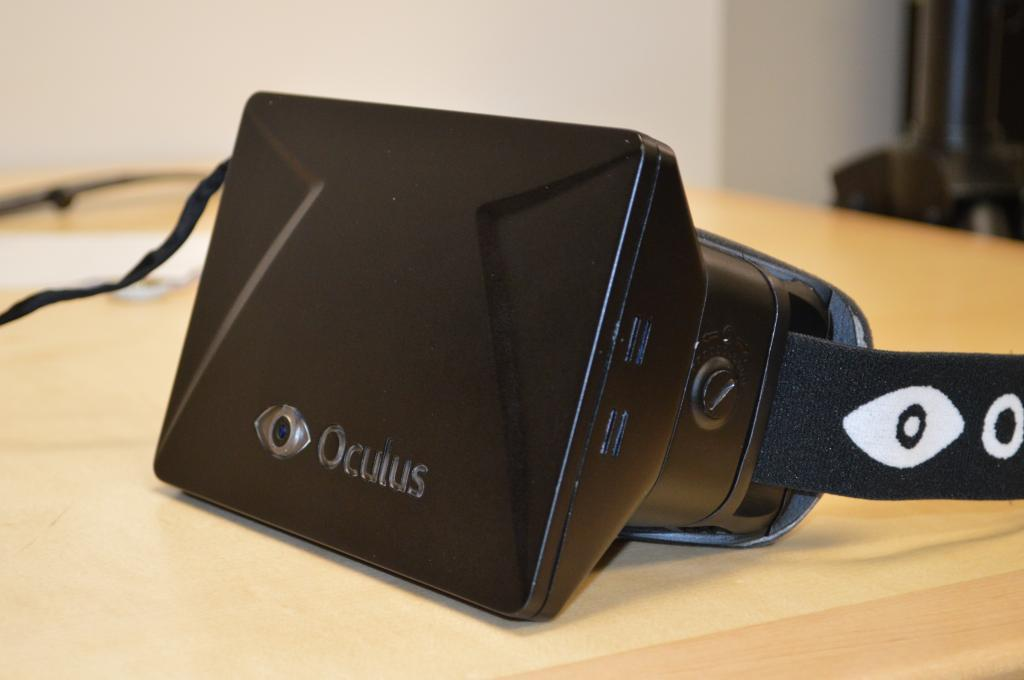
\includegraphics[width=0.5\textwidth]{oculus.jpg}
\caption{Oculus Rift Development Kit 1. 
\cite{website:pcworld}}
\label{fig:oculus}
\end{figure}

\begin{figure}[]
\centering
\includegraphics[width=0.5\textwidth]{stereo_lens.png}
\caption{Above is a stereoscopic split screen view also rendered with barrel distortion.
    Below, are the magnifying lenses of the oculus headset.
Frames displayed on the Oculus screen appear normal when the headset is worn.}
\label{fig:stereo}
\end{figure}


The Oculus Rift seen in Fig. \ref{fig:oculus} is the current state of the art
in HMD VR technology. There are several elements to the device that allow the
Oculus to provide the most immersive visual VR experience thus seen.

The first is speed.  The VR realism is directly tied to this response time and
the Oculus overcomes the problem of graphical latency, which has plagued all of
its predecessors, by sampling data from its 3-axis gyro, accelerometers, and
magnetometers at a rate of 250Hz \cite{website:roadtovr}; the newer version is
said to have a sampling rate of 1000Hz. Its ability to gather data so quickly
from its propriocetive sensors allows the graphics on the display to be
adjusted to correspond to real time head movements. Secondly, the Oculus
renders scenes split screen stereoscopic 3D. The left eye sees the left half of
the screen and the right eye sees the right half, which is consistent with
human perception. Leveraging split screen stereo greatly enhances the perceived
3D effect. Finally, the Oculus uses large magnifying lenses in order to
completely encompass the user's peripheral vision and greatly expand field of
view. All of these aspects must be considered when developing the graphics of
the scene. Fortunately the SDK provides sufficient overhead to deal with them,
allowing graphics developers to stay focused on developing graphics instead of
worrying about the details of implementation.

The most simple applications one can develop for the Oculus are created using
basic OpenGL. The only caveat being that a separate framebuffer must be bound
to the context for off-screen rendering. The framebuffer must have a texture
bound to at as well which will be written to at the last stage of the
conventional pipeline. Parameters for constructing the texture are provided
directly from the Oculus SDK programmatically. The Oculus SDK will then take the
data placed in the texture and perform the post-processing for stereoscopic 3D
rendering and distortion processing. 

Human eye pupils are approximately 65 mm apart.  This interpupillary distance
(IPD) must be taken into consideration for configuring the in-application
camera. Therefore, each scene is rendered twice, once for the virtual camera
on the left, and once for the virtual camera on the right. Both of which are
subject to a translation with respect to one another causing the stereoscopic
effect. 

The use of the large magnifying lenses causes the image succumbs to a great
deal of pincushion distortion. To rectify this distortion, the software must
apply an equal and opposite amount of barrel distortion. The final image
rendered to the Oculus's display can be seen in Fig. \ref{fig:stereo}. For the
remainder of this paper, when discussing the camera view, this refers to the
single camera model provided to the Oculus SDK before the post processing
occurs. 

However, the Oculus is not without limitations. While it is able to track
rotation effectively, it provides no means of tracking translation. Those
familiar with the company should find themselves critical, as they know that
the newer version of the Oculus does provides position tracking as well. Be
that as it may, its position tracking is limited as it is designed to track
within a small volumes, say the space in front of a desk. In addition, it
provides not ability track any other objects other than itself.

Graphics is known as the inverse problem to computer vision. Where computer
vision seeks to extract information about an environment from an image,
graphics seeks to extract information to construct an image from an
environment. What gives computer graphics the illusion of position and depth is
a mathematical process of constructing a series of transformations taking
arbitrary points from one frame of reference to another to infer position and
ultimately a projective transform to infer depth. The location of all the
particles in an object can be defined with respect to some inertial frame of
reference. If one observes the object from some alternative location and
orientation with respect to the same inertial frame, one can construct a
transformation to take points from the inertial frame to the view frame.
Ultimately, all the objects in the scene must be transformed from their own
respective frames of reference to this view frame. Manipulating the pose of
this view frame is what we are interested in. Normally, the orientation of
the Oculus is constructed from the measurements provided by its sensors,
and is used directly as the orientation of the view frame.

\begin{figure}[]
\centering
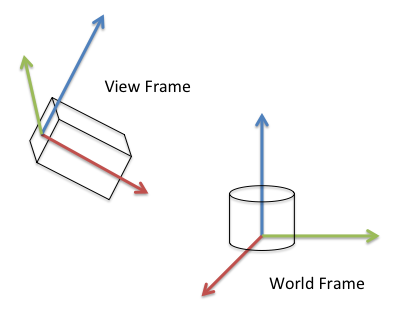
\includegraphics[width=0.5\textwidth]{world_view.png}
\caption{Two frames of reference, the view and the world. The orientation and
position of the view frame corresponds to the camera view. The axis are
defined in the graphics convention. Red is \emph{x}, green is \emph{y}, 
and blue is \emph{z}.}
\label{fig:worldview}
\end{figure}



\bibliographystyle{IEEEtran}
\bibliography{IEEEabrv,bibliography}

\end{document}
